% Options for packages loaded elsewhere
\PassOptionsToPackage{unicode}{hyperref}
\PassOptionsToPackage{hyphens}{url}
%
\documentclass[
]{book}
\usepackage{lmodern}
\usepackage{setspace}
\usepackage{amssymb,amsmath}
\usepackage{ifxetex,ifluatex}
\ifnum 0\ifxetex 1\fi\ifluatex 1\fi=0 % if pdftex
  \usepackage[T1]{fontenc}
  \usepackage[utf8]{inputenc}
  \usepackage{textcomp} % provide euro and other symbols
\else % if luatex or xetex
  \usepackage{unicode-math}
  \defaultfontfeatures{Scale=MatchLowercase}
  \defaultfontfeatures[\rmfamily]{Ligatures=TeX,Scale=1}
\fi
% Use upquote if available, for straight quotes in verbatim environments
\IfFileExists{upquote.sty}{\usepackage{upquote}}{}
\IfFileExists{microtype.sty}{% use microtype if available
  \usepackage[]{microtype}
  \UseMicrotypeSet[protrusion]{basicmath} % disable protrusion for tt fonts
}{}
\makeatletter
\@ifundefined{KOMAClassName}{% if non-KOMA class
  \IfFileExists{parskip.sty}{%
    \usepackage{parskip}
  }{% else
    \setlength{\parindent}{0pt}
    \setlength{\parskip}{6pt plus 2pt minus 1pt}}
}{% if KOMA class
  \KOMAoptions{parskip=half}}
\makeatother
\usepackage{xcolor}
\IfFileExists{xurl.sty}{\usepackage{xurl}}{} % add URL line breaks if available
\IfFileExists{bookmark.sty}{\usepackage{bookmark}}{\usepackage{hyperref}}
\hypersetup{
  pdftitle={Office of Student Financial Aid},
  pdfauthor={Glen C. Falk},
  hidelinks,
  pdfcreator={LaTeX via pandoc}}
\urlstyle{same} % disable monospaced font for URLs
\usepackage{color}
\usepackage{fancyvrb}
\newcommand{\VerbBar}{|}
\newcommand{\VERB}{\Verb[commandchars=\\\{\}]}
\DefineVerbatimEnvironment{Highlighting}{Verbatim}{commandchars=\\\{\}}
% Add ',fontsize=\small' for more characters per line
\usepackage{framed}
\definecolor{shadecolor}{RGB}{248,248,248}
\newenvironment{Shaded}{\begin{snugshade}}{\end{snugshade}}
\newcommand{\AlertTok}[1]{\textcolor[rgb]{0.94,0.16,0.16}{#1}}
\newcommand{\AnnotationTok}[1]{\textcolor[rgb]{0.56,0.35,0.01}{\textbf{\textit{#1}}}}
\newcommand{\AttributeTok}[1]{\textcolor[rgb]{0.77,0.63,0.00}{#1}}
\newcommand{\BaseNTok}[1]{\textcolor[rgb]{0.00,0.00,0.81}{#1}}
\newcommand{\BuiltInTok}[1]{#1}
\newcommand{\CharTok}[1]{\textcolor[rgb]{0.31,0.60,0.02}{#1}}
\newcommand{\CommentTok}[1]{\textcolor[rgb]{0.56,0.35,0.01}{\textit{#1}}}
\newcommand{\CommentVarTok}[1]{\textcolor[rgb]{0.56,0.35,0.01}{\textbf{\textit{#1}}}}
\newcommand{\ConstantTok}[1]{\textcolor[rgb]{0.00,0.00,0.00}{#1}}
\newcommand{\ControlFlowTok}[1]{\textcolor[rgb]{0.13,0.29,0.53}{\textbf{#1}}}
\newcommand{\DataTypeTok}[1]{\textcolor[rgb]{0.13,0.29,0.53}{#1}}
\newcommand{\DecValTok}[1]{\textcolor[rgb]{0.00,0.00,0.81}{#1}}
\newcommand{\DocumentationTok}[1]{\textcolor[rgb]{0.56,0.35,0.01}{\textbf{\textit{#1}}}}
\newcommand{\ErrorTok}[1]{\textcolor[rgb]{0.64,0.00,0.00}{\textbf{#1}}}
\newcommand{\ExtensionTok}[1]{#1}
\newcommand{\FloatTok}[1]{\textcolor[rgb]{0.00,0.00,0.81}{#1}}
\newcommand{\FunctionTok}[1]{\textcolor[rgb]{0.00,0.00,0.00}{#1}}
\newcommand{\ImportTok}[1]{#1}
\newcommand{\InformationTok}[1]{\textcolor[rgb]{0.56,0.35,0.01}{\textbf{\textit{#1}}}}
\newcommand{\KeywordTok}[1]{\textcolor[rgb]{0.13,0.29,0.53}{\textbf{#1}}}
\newcommand{\NormalTok}[1]{#1}
\newcommand{\OperatorTok}[1]{\textcolor[rgb]{0.81,0.36,0.00}{\textbf{#1}}}
\newcommand{\OtherTok}[1]{\textcolor[rgb]{0.56,0.35,0.01}{#1}}
\newcommand{\PreprocessorTok}[1]{\textcolor[rgb]{0.56,0.35,0.01}{\textit{#1}}}
\newcommand{\RegionMarkerTok}[1]{#1}
\newcommand{\SpecialCharTok}[1]{\textcolor[rgb]{0.00,0.00,0.00}{#1}}
\newcommand{\SpecialStringTok}[1]{\textcolor[rgb]{0.31,0.60,0.02}{#1}}
\newcommand{\StringTok}[1]{\textcolor[rgb]{0.31,0.60,0.02}{#1}}
\newcommand{\VariableTok}[1]{\textcolor[rgb]{0.00,0.00,0.00}{#1}}
\newcommand{\VerbatimStringTok}[1]{\textcolor[rgb]{0.31,0.60,0.02}{#1}}
\newcommand{\WarningTok}[1]{\textcolor[rgb]{0.56,0.35,0.01}{\textbf{\textit{#1}}}}
\usepackage{longtable,booktabs}
% Correct order of tables after \paragraph or \subparagraph
\usepackage{etoolbox}
\makeatletter
\patchcmd\longtable{\par}{\if@noskipsec\mbox{}\fi\par}{}{}
\makeatother
% Allow footnotes in longtable head/foot
\IfFileExists{footnotehyper.sty}{\usepackage{footnotehyper}}{\usepackage{footnote}}
\makesavenoteenv{longtable}
\usepackage{graphicx,grffile}
\makeatletter
\def\maxwidth{\ifdim\Gin@nat@width>\linewidth\linewidth\else\Gin@nat@width\fi}
\def\maxheight{\ifdim\Gin@nat@height>\textheight\textheight\else\Gin@nat@height\fi}
\makeatother
% Scale images if necessary, so that they will not overflow the page
% margins by default, and it is still possible to overwrite the defaults
% using explicit options in \includegraphics[width, height, ...]{}
\setkeys{Gin}{width=\maxwidth,height=\maxheight,keepaspectratio}
% Set default figure placement to htbp
\makeatletter
\def\fps@figure{htbp}
\makeatother
% Make links footnotes instead of hotlinks:
\DeclareRobustCommand{\href}[2]{#2\footnote{\url{#1}}}
\setlength{\emergencystretch}{3em} % prevent overfull lines
\providecommand{\tightlist}{%
  \setlength{\itemsep}{0pt}\setlength{\parskip}{0pt}}
\setcounter{secnumdepth}{5}
\usepackage{booktabs}
\usepackage{booktabs}
\usepackage{longtable}
\usepackage{array}
\usepackage{multirow}
\usepackage{wrapfig}
\usepackage{float}
\usepackage{colortbl}
\usepackage{pdflscape}
\usepackage{tabu}
\usepackage{threeparttable}
\usepackage{threeparttablex}
\usepackage[normalem]{ulem}
\usepackage{makecell}
\usepackage{xcolor}
\usepackage{amsmath}
\usepackage{caption}
\usepackage[]{natbib}
\bibliographystyle{apalike}

\title{Office of Student Financial Aid}
\usepackage{etoolbox}
\makeatletter
\providecommand{\subtitle}[1]{% add subtitle to \maketitle
  \apptocmd{\@title}{\par {\large #1 \par}}{}{}
}
\makeatother
\subtitle{Annual Reports}
\author{Glen C. Falk}
\date{2020-03-10}

\begin{document}
\maketitle

{
\setcounter{tocdepth}{1}
\tableofcontents
}
\setstretch{1.15}
\hypertarget{osfa-org-chart}{%
\chapter*{OSFA Org Chart}\label{osfa-org-chart}}
\addcontentsline{toc}{chapter}{OSFA Org Chart}

Here is the current OSFA Organization chart.

\begin{figure}

{\centering 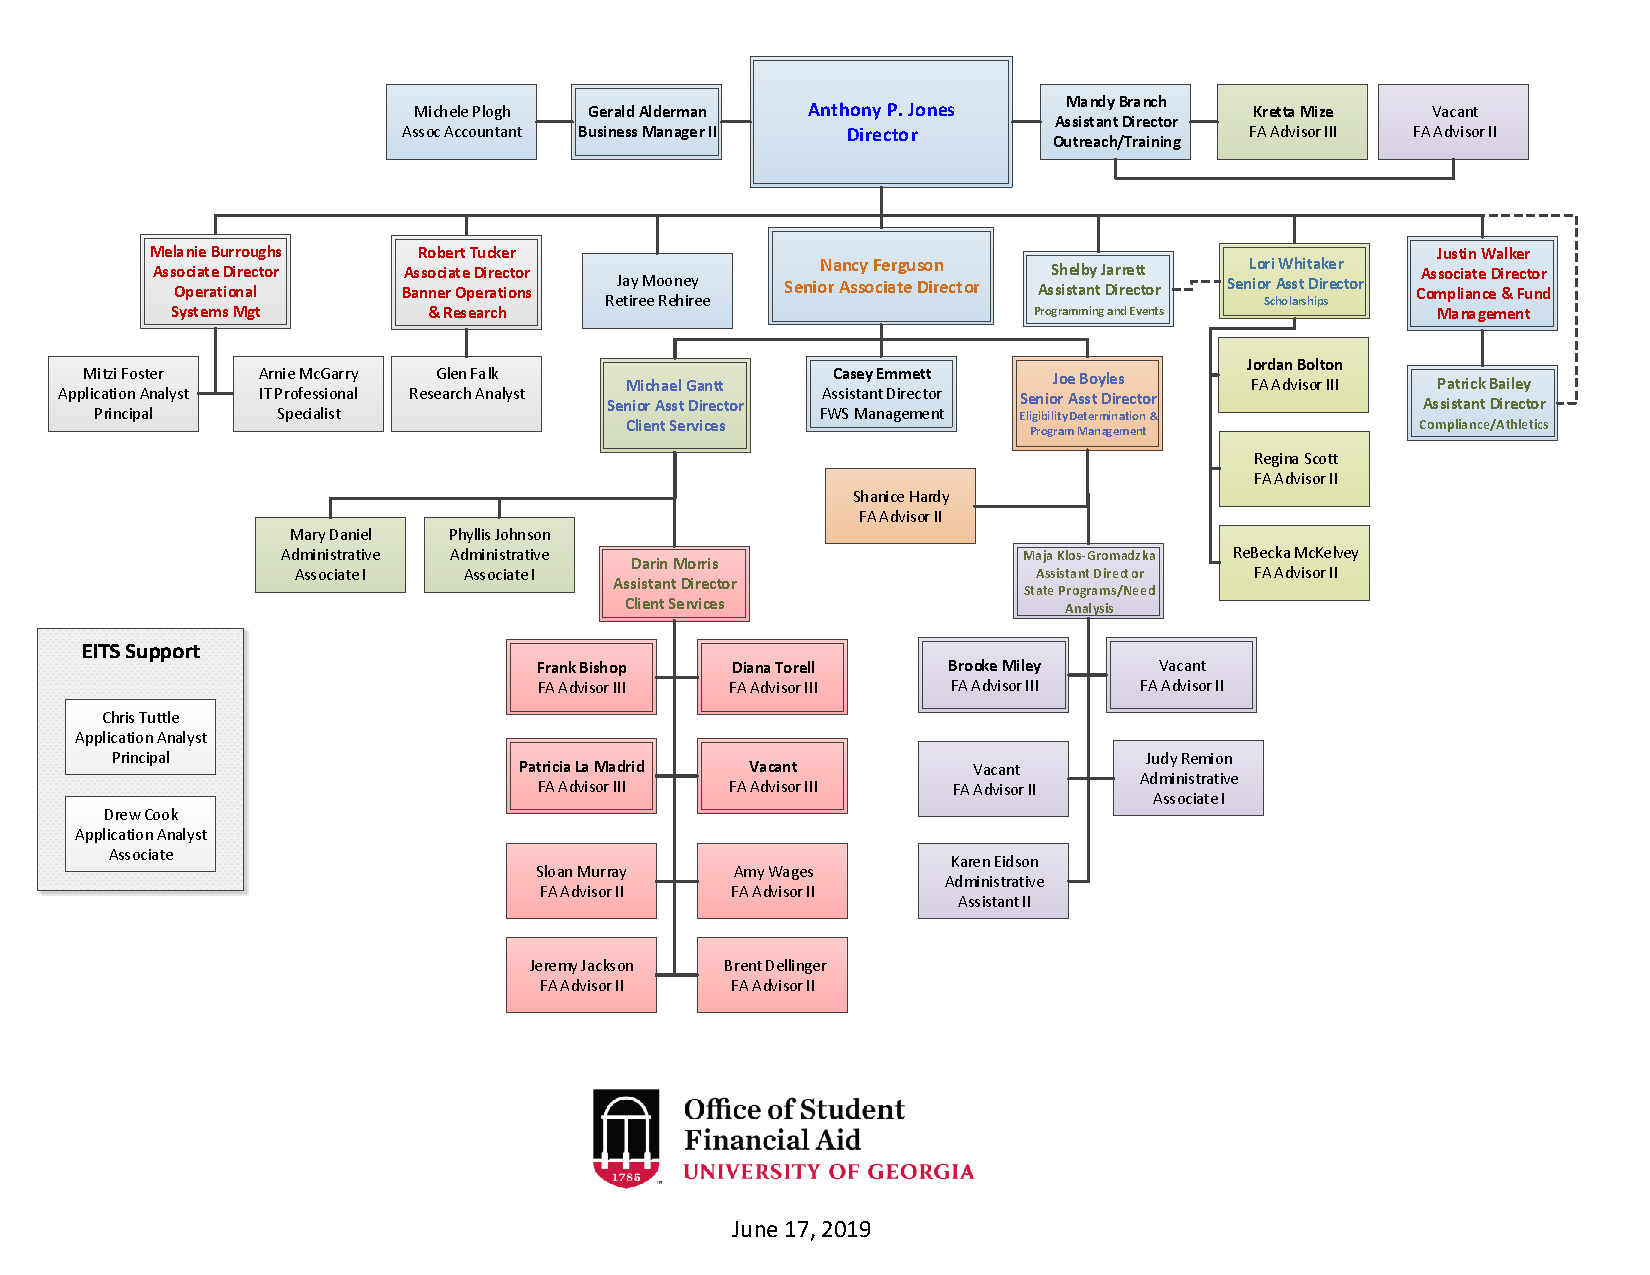
\includegraphics[width=1\linewidth]{images/OSFAOrgChart} 

}

\caption{OSFA Org Chart}\label{fig:label}
\end{figure}

\hypertarget{intro}{%
\chapter{01. Student Financial Aid Summary}\label{intro}}

You can label chapter and section titles using \texttt{\{\#label\}} after them, e.g., we can reference Chapter \ref{intro}. If you do not manually label them, there will be automatic labels anyway, e.g., Chapter \ref{methods}.

Figures and tables with captions will be placed in \texttt{figure} and \texttt{table} environments, respectively.

\begin{Shaded}
\begin{Highlighting}[]
\KeywordTok{par}\NormalTok{(}\DataTypeTok{mar =} \KeywordTok{c}\NormalTok{(}\DecValTok{4}\NormalTok{, }\DecValTok{4}\NormalTok{, }\FloatTok{.1}\NormalTok{, }\FloatTok{.1}\NormalTok{))}
\KeywordTok{plot}\NormalTok{(pressure, }\DataTypeTok{type =} \StringTok{'b'}\NormalTok{, }\DataTypeTok{pch =} \DecValTok{19}\NormalTok{)}
\end{Highlighting}
\end{Shaded}

\begin{figure}

{\centering 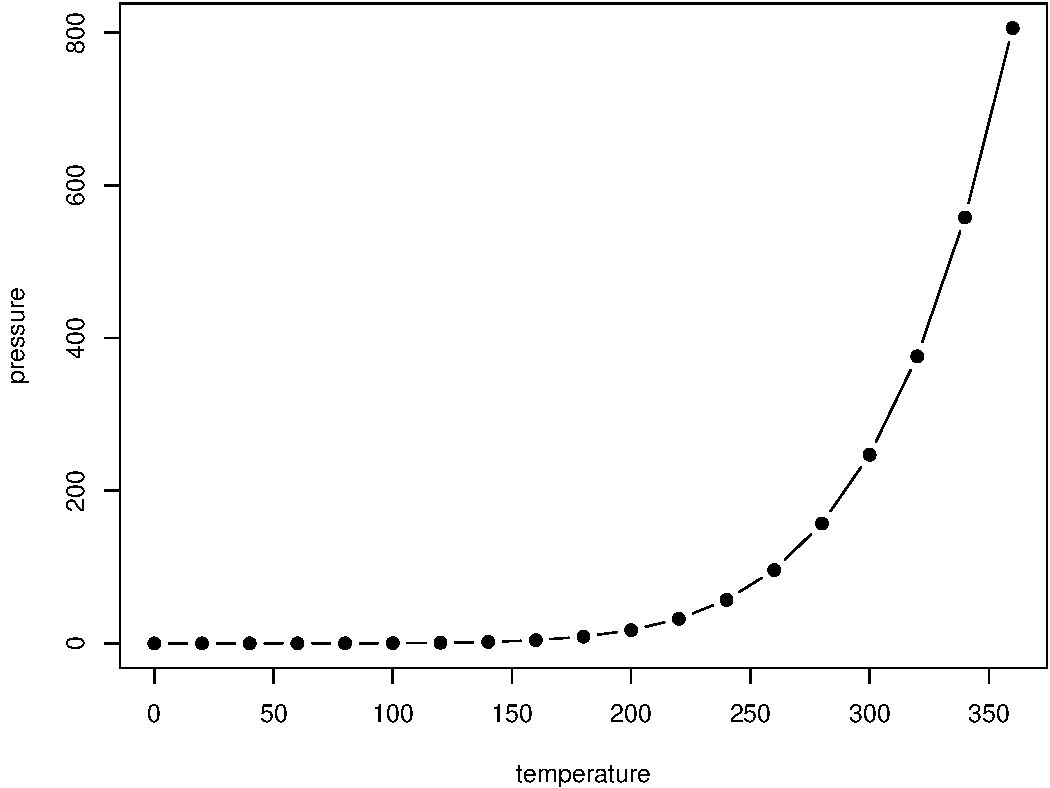
\includegraphics[width=0.8\linewidth]{01-Student-Financial-Aid-Summary_files/figure-latex/nice-fig-1} 

}

\caption{Here is a nice figure!}\label{fig:nice-fig}
\end{figure}

Reference a figure by its code chunk label with the \texttt{fig:} prefix, e.g., see Figure \ref{fig:nice-fig}. Similarly, you can reference tables generated from \texttt{knitr::kable()}, e.g., see Table \ref{tab:nice-tab}.

\begin{Shaded}
\begin{Highlighting}[]
\NormalTok{knitr}\OperatorTok{::}\KeywordTok{kable}\NormalTok{(}
  \KeywordTok{head}\NormalTok{(iris, }\DecValTok{20}\NormalTok{), }\DataTypeTok{caption =} \StringTok{'Here is a nice table!'}\NormalTok{,}
  \DataTypeTok{booktabs =} \OtherTok{TRUE}
\NormalTok{)}
\end{Highlighting}
\end{Shaded}

\begin{table}

\caption{\label{tab:nice-tab}Here is a nice table!}
\centering
\begin{tabular}[t]{rrrrl}
\toprule
Sepal.Length & Sepal.Width & Petal.Length & Petal.Width & Species\\
\midrule
5.1 & 3.5 & 1.4 & 0.2 & setosa\\
4.9 & 3.0 & 1.4 & 0.2 & setosa\\
4.7 & 3.2 & 1.3 & 0.2 & setosa\\
4.6 & 3.1 & 1.5 & 0.2 & setosa\\
5.0 & 3.6 & 1.4 & 0.2 & setosa\\
\addlinespace
5.4 & 3.9 & 1.7 & 0.4 & setosa\\
4.6 & 3.4 & 1.4 & 0.3 & setosa\\
5.0 & 3.4 & 1.5 & 0.2 & setosa\\
4.4 & 2.9 & 1.4 & 0.2 & setosa\\
4.9 & 3.1 & 1.5 & 0.1 & setosa\\
\addlinespace
5.4 & 3.7 & 1.5 & 0.2 & setosa\\
4.8 & 3.4 & 1.6 & 0.2 & setosa\\
4.8 & 3.0 & 1.4 & 0.1 & setosa\\
4.3 & 3.0 & 1.1 & 0.1 & setosa\\
5.8 & 4.0 & 1.2 & 0.2 & setosa\\
\addlinespace
5.7 & 4.4 & 1.5 & 0.4 & setosa\\
5.4 & 3.9 & 1.3 & 0.4 & setosa\\
5.1 & 3.5 & 1.4 & 0.3 & setosa\\
5.7 & 3.8 & 1.7 & 0.3 & setosa\\
5.1 & 3.8 & 1.5 & 0.3 & setosa\\
\bottomrule
\end{tabular}
\end{table}

You can write citations, too. For example, we are using the \textbf{bookdown} package \citep{R-bookdown} in this sample book, which was built on top of R Markdown and \textbf{knitr} \citep{xie2015}.

\hypertarget{coa}{%
\chapter{COA}\label{coa}}

\hypertarget{coa-tables}{%
\section{COA Tables}\label{coa-tables}}

\hypertarget{example-one---flextable}{%
\subsection{Example one - flextable}\label{example-one---flextable}}

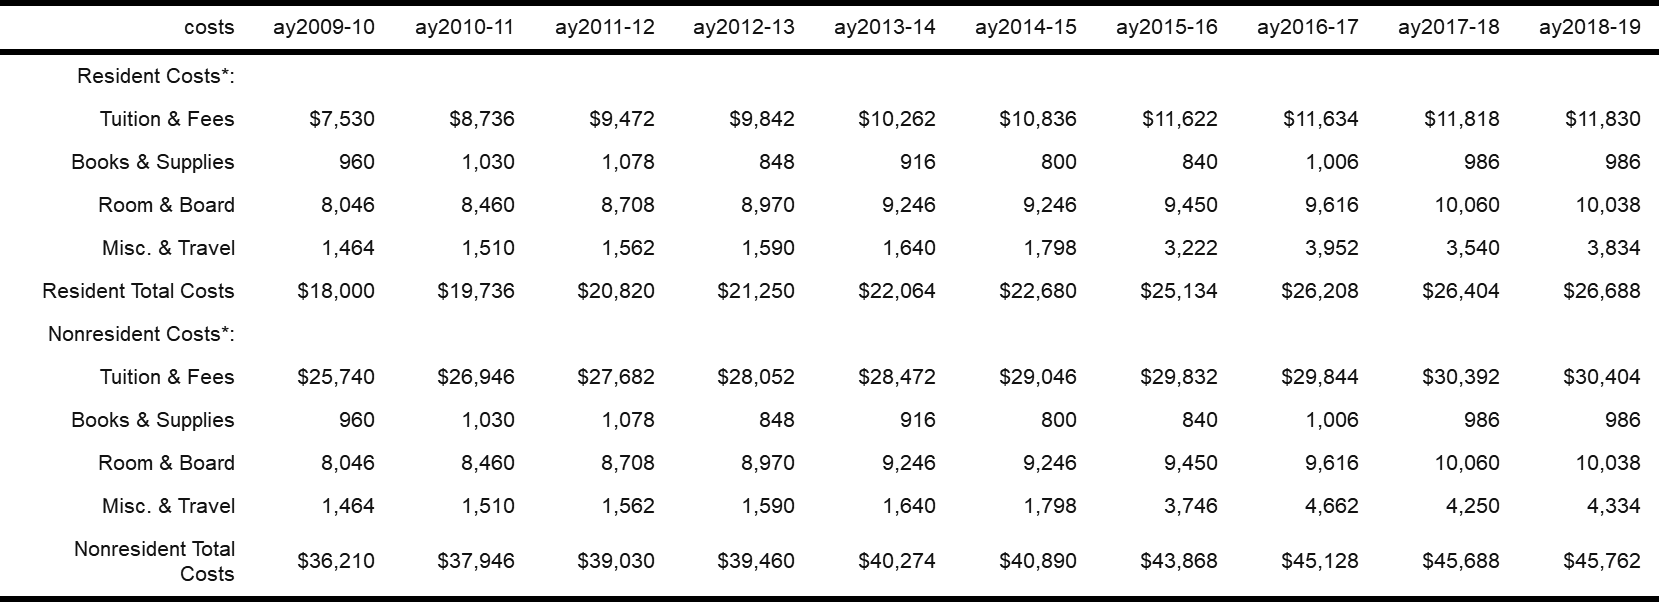
\includegraphics[width=7.67in,height=2.07in,keepaspectratio]{02-COA_files/figure-latex/2.1.1-coa-flextable-1.png}

\hypertarget{example-two---gt}{%
\subsection{Example two - gt}\label{example-two---gt}}

\captionsetup[table]{labelformat=empty,skip=1pt}
\begin{longtable}{lllllllllll}
\caption*{
\large COA\\ 
\small Undergrad\\ 
} \\ 
\toprule
costs & ay2009-10 & ay2010-11 & ay2011-12 & ay2012-13 & ay2013-14 & ay2014-15 & ay2015-16 & ay2016-17 & ay2017-18 & ay2018-19 \\ 
\midrule
Resident Costs*: &  &  &  &  &  &  &  &  &  &  \\ 
Tuition \& Fees & \$7,530 & \$8,736 & \$9,472 & \$9,842 & \$10,262 & \$10,836 & \$11,622 & \$11,634 & \$11,818 & \$11,830 \\ 
Books \& Supplies & 960 & 1,030 & 1,078 & 848 & 916 & 800 & 840 & 1,006 & 986 & 986 \\ 
Room \& Board & 8,046 & 8,460 & 8,708 & 8,970 & 9,246 & 9,246 & 9,450 & 9,616 & 10,060 & 10,038 \\ 
Misc. \& Travel & 1,464 & 1,510 & 1,562 & 1,590 & 1,640 & 1,798 & 3,222 & 3,952 & 3,540 & 3,834 \\ 
Resident Total Costs & \$18,000 & \$19,736 & \$20,820 & \$21,250 & \$22,064 & \$22,680 & \$25,134 & \$26,208 & \$26,404 & \$26,688 \\ 
Nonresident Costs*: &  &  &  &  &  &  &  &  &  &  \\ 
Tuition \& Fees & \$25,740 & \$26,946 & \$27,682 & \$28,052 & \$28,472 & \$29,046 & \$29,832 & \$29,844 & \$30,392 & \$30,404 \\ 
Books \& Supplies & 960 & 1,030 & 1,078 & 848 & 916 & 800 & 840 & 1,006 & 986 & 986 \\ 
Room \& Board & 8,046 & 8,460 & 8,708 & 8,970 & 9,246 & 9,246 & 9,450 & 9,616 & 10,060 & 10,038 \\ 
Misc. \& Travel & 1,464 & 1,510 & 1,562 & 1,590 & 1,640 & 1,798 & 3,746 & 4,662 & 4,250 & 4,334 \\ 
Nonresident Total Costs & \$36,210 & \$37,946 & \$39,030 & \$39,460 & \$40,274 & \$40,890 & \$43,868 & \$45,128 & \$45,688 & \$45,762 \\ 
\bottomrule
\end{longtable}

\hypertarget{example-three---kable}{%
\subsection{Example three - kable}\label{example-three---kable}}

\begin{tabular}{l|l|l|l|l|l|l|l|l|l|l}
\hline
costs & ay2009-10 & ay2010-11 & ay2011-12 & ay2012-13 & ay2013-14 & ay2014-15 & ay2015-16 & ay2016-17 & ay2017-18 & ay2018-19\\
\hline
Resident Costs*: &  &  &  &  &  &  &  &  &  & \\
\hline
Tuition \& Fees & \$7,530 & \$8,736 & \$9,472 & \$9,842 & \$10,262 & \$10,836 & \$11,622 & \$11,634 & \$11,818 & \$11,830\\
\hline
Books \& Supplies & 960 & 1,030 & 1,078 & 848 & 916 & 800 & 840 & 1,006 & 986 & 986\\
\hline
Room \& Board & 8,046 & 8,460 & 8,708 & 8,970 & 9,246 & 9,246 & 9,450 & 9,616 & 10,060 & 10,038\\
\hline
Misc. \& Travel & 1,464 & 1,510 & 1,562 & 1,590 & 1,640 & 1,798 & 3,222 & 3,952 & 3,540 & 3,834\\
\hline
Resident Total Costs & \$18,000 & \$19,736 & \$20,820 & \$21,250 & \$22,064 & \$22,680 & \$25,134 & \$26,208 & \$26,404 & \$26,688\\
\hline
Nonresident Costs*: &  &  &  &  &  &  &  &  &  & \\
\hline
Tuition \& Fees & \$25,740 & \$26,946 & \$27,682 & \$28,052 & \$28,472 & \$29,046 & \$29,832 & \$29,844 & \$30,392 & \$30,404\\
\hline
Books \& Supplies & 960 & 1,030 & 1,078 & 848 & 916 & 800 & 840 & 1,006 & 986 & 986\\
\hline
Room \& Board & 8,046 & 8,460 & 8,708 & 8,970 & 9,246 & 9,246 & 9,450 & 9,616 & 10,060 & 10,038\\
\hline
Misc. \& Travel & 1,464 & 1,510 & 1,562 & 1,590 & 1,640 & 1,798 & 3,746 & 4,662 & 4,250 & 4,334\\
\hline
Nonresident Total Costs & \$36,210 & \$37,946 & \$39,030 & \$39,460 & \$40,274 & \$40,890 & \$43,868 & \$45,128 & \$45,688 & \$45,762\\
\hline
\end{tabular}

\begin{tabular}{l|l|l|l|l|l|l|l|l|l|l}
\hline
costs & ay2009-10 & ay2010-11 & ay2011-12 & ay2012-13 & ay2013-14 & ay2014-15 & ay2015-16 & ay2016-17 & ay2017-18 & ay2018-19\\
\hline
Resident Costs*: &  &  &  &  &  &  &  &  &  & \\
\hline
Tuition \& Fees & \$7,530 & \$8,736 & \$9,472 & \$9,842 & \$10,262 & \$10,836 & \$11,622 & \$11,634 & \$11,818 & \$11,830\\
\hline
Books \& Supplies & 960 & 1,030 & 1,078 & 848 & 916 & 800 & 840 & 1,006 & 986 & 986\\
\hline
Room \& Board & 8,046 & 8,460 & 8,708 & 8,970 & 9,246 & 9,246 & 9,450 & 9,616 & 10,060 & 10,038\\
\hline
Misc. \& Travel & 1,464 & 1,510 & 1,562 & 1,590 & 1,640 & 1,798 & 3,222 & 3,952 & 3,540 & 3,834\\
\hline
Resident Total Costs & \$18,000 & \$19,736 & \$20,820 & \$21,250 & \$22,064 & \$22,680 & \$25,134 & \$26,208 & \$26,404 & \$26,688\\
\hline
Nonresident Costs*: &  &  &  &  &  &  &  &  &  & \\
\hline
Tuition \& Fees & \$25,740 & \$26,946 & \$27,682 & \$28,052 & \$28,472 & \$29,046 & \$29,832 & \$29,844 & \$30,392 & \$30,404\\
\hline
Books \& Supplies & 960 & 1,030 & 1,078 & 848 & 916 & 800 & 840 & 1,006 & 986 & 986\\
\hline
Room \& Board & 8,046 & 8,460 & 8,708 & 8,970 & 9,246 & 9,246 & 9,450 & 9,616 & 10,060 & 10,038\\
\hline
Misc. \& Travel & 1,464 & 1,510 & 1,562 & 1,590 & 1,640 & 1,798 & 3,746 & 4,662 & 4,250 & 4,334\\
\hline
Nonresident Total Costs & \$36,210 & \$37,946 & \$39,030 & \$39,460 & \$40,274 & \$40,890 & \$43,868 & \$45,128 & \$45,688 & \$45,762\\
\hline
\end{tabular}

\hypertarget{example-four---xtable}{%
\subsection{Example four - xtable}\label{example-four---xtable}}

\begin{verbatim}
## % latex table generated in R 3.6.3 by xtable 1.8-4 package
## % Tue Mar 10 07:20:01 2020
## \begin{table}[ht]
## \centering
## \begin{tabular}{}
##   \toprule
##  & costs & ay2009-10 & ay2010-11 & ay2011-12 & ay2012-13 & ay2013-14 & ay2014-15 & ay2015-16 & ay2016-17 & ay2017-18 & ay2018-19 \\ 
##   \midrule
## 1 & Resident Costs*: &  &  &  &  &  &  &  &  &  &  \\ 
##   2 & Tuition \& Fees & \$7,530 & \$8,736 & \$9,472 & \$9,842 & \$10,262 & \$10,836 & \$11,622 & \$11,634 & \$11,818 & \$11,830 \\ 
##   3 & Books \& Supplies & 960 & 1,030 & 1,078 & 848 & 916 & 800 & 840 & 1,006 & 986 & 986 \\ 
##   4 & Room \& Board & 8,046 & 8,460 & 8,708 & 8,970 & 9,246 & 9,246 & 9,450 & 9,616 & 10,060 & 10,038 \\ 
##   5 & Misc. \& Travel & 1,464 & 1,510 & 1,562 & 1,590 & 1,640 & 1,798 & 3,222 & 3,952 & 3,540 & 3,834 \\ 
##   6 & Resident Total Costs & \$18,000 & \$19,736 & \$20,820 & \$21,250 & \$22,064 & \$22,680 & \$25,134 & \$26,208 & \$26,404 & \$26,688 \\ 
##   7 & Nonresident Costs*: &  &  &  &  &  &  &  &  &  &  \\ 
##   8 & Tuition \& Fees & \$25,740 & \$26,946 & \$27,682 & \$28,052 & \$28,472 & \$29,046 & \$29,832 & \$29,844 & \$30,392 & \$30,404 \\ 
##   9 & Books \& Supplies & 960 & 1,030 & 1,078 & 848 & 916 & 800 & 840 & 1,006 & 986 & 986 \\ 
##   10 & Room \& Board & 8,046 & 8,460 & 8,708 & 8,970 & 9,246 & 9,246 & 9,450 & 9,616 & 10,060 & 10,038 \\ 
##   11 & Misc. \& Travel & 1,464 & 1,510 & 1,562 & 1,590 & 1,640 & 1,798 & 3,746 & 4,662 & 4,250 & 4,334 \\ 
##   12 & Nonresident Total Costs & \$36,210 & \$37,946 & \$39,030 & \$39,460 & \$40,274 & \$40,890 & \$43,868 & \$45,128 & \$45,688 & \$45,762 \\ 
##    \bottomrule
## \end{tabular}
## \end{table}
\end{verbatim}

\hypertarget{coa-charts}{%
\section{COA Charts}\label{coa-charts}}

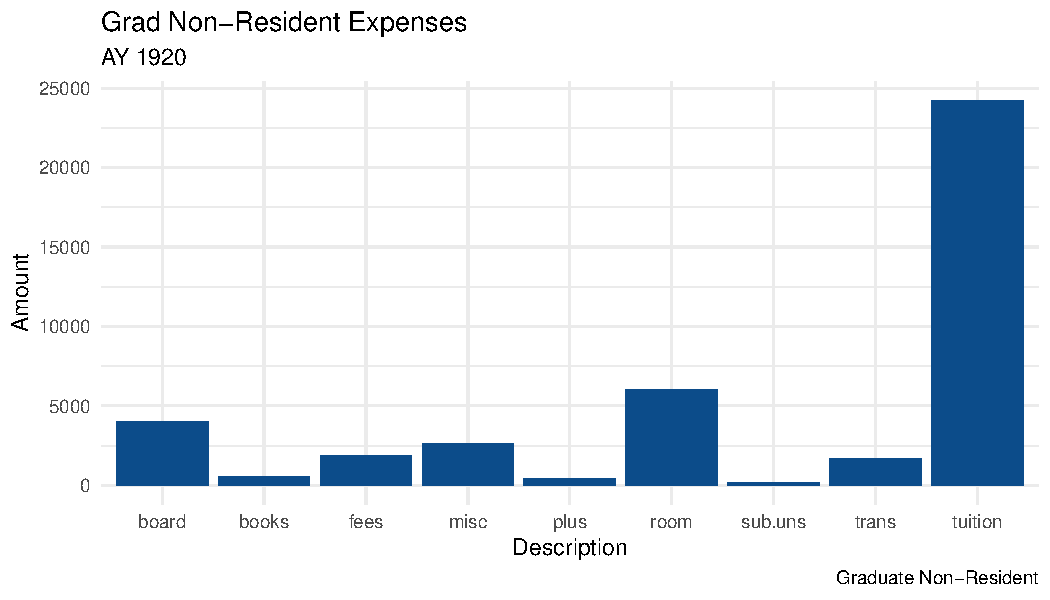
\includegraphics{02-COA_files/figure-latex/2.2.1-coa-non-1.pdf}

\begin{figure}
\centering
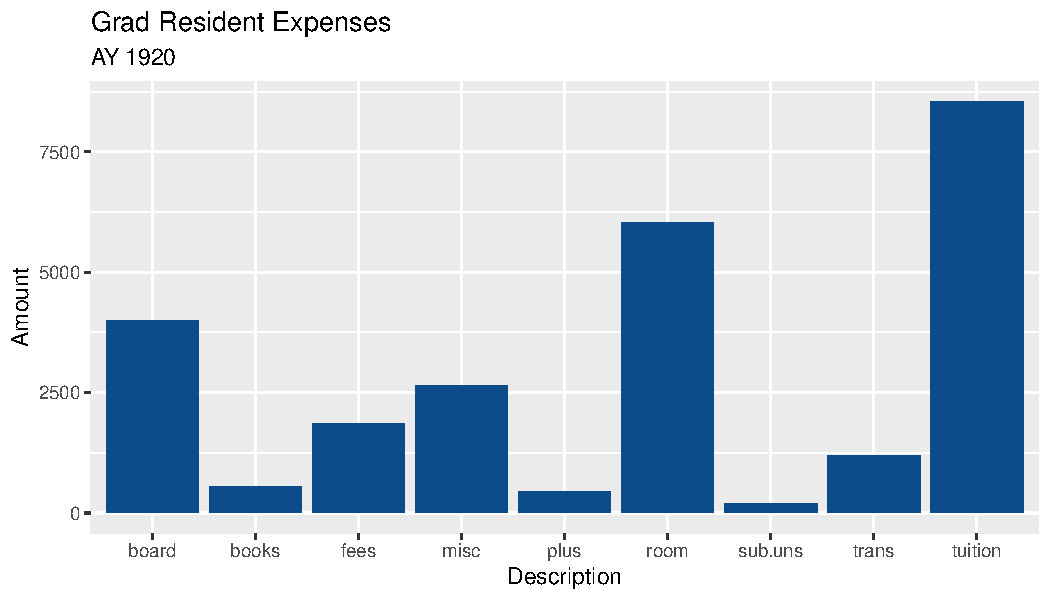
\includegraphics{02-COA_files/figure-latex/2.2.2-coa-res-1.pdf}
\caption{(\#fig:2.2.2-coa-res)coa-res}
\end{figure}

\begin{figure}
\centering
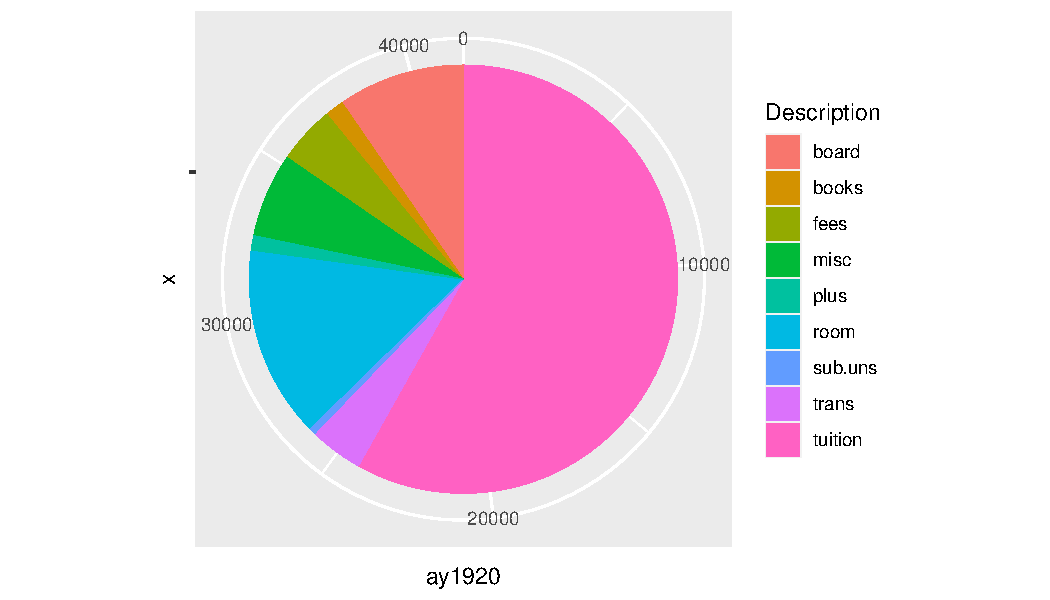
\includegraphics{02-COA_files/figure-latex/2.2.3-coa-non-1.pdf}
\caption{(\#fig:2.2.3-coa-non)coa-grad-non-pie}
\end{figure}

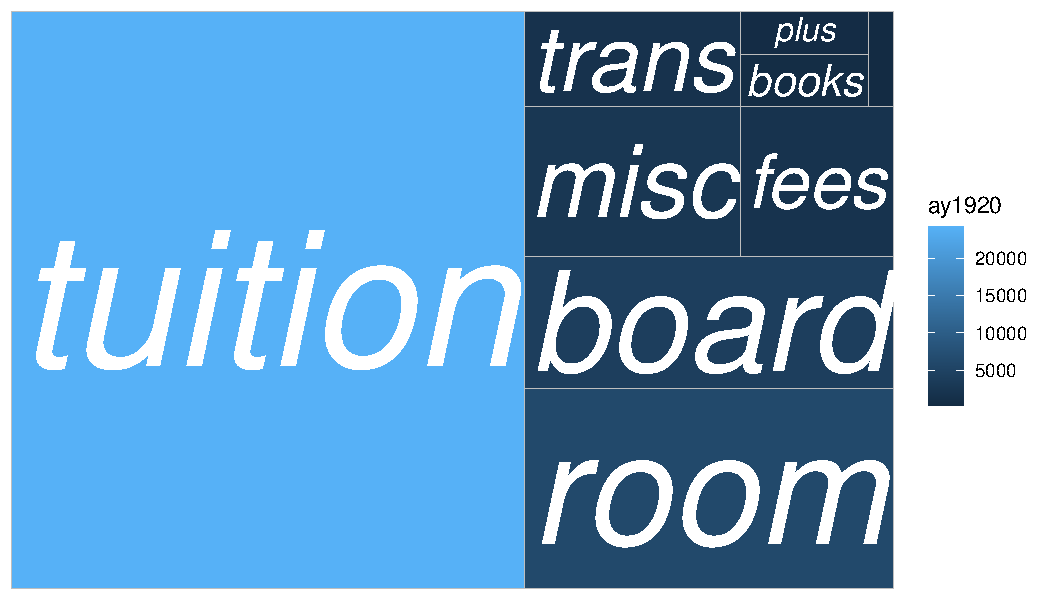
\includegraphics{02-COA_files/figure-latex/2.2.4-coa-non-1.pdf}
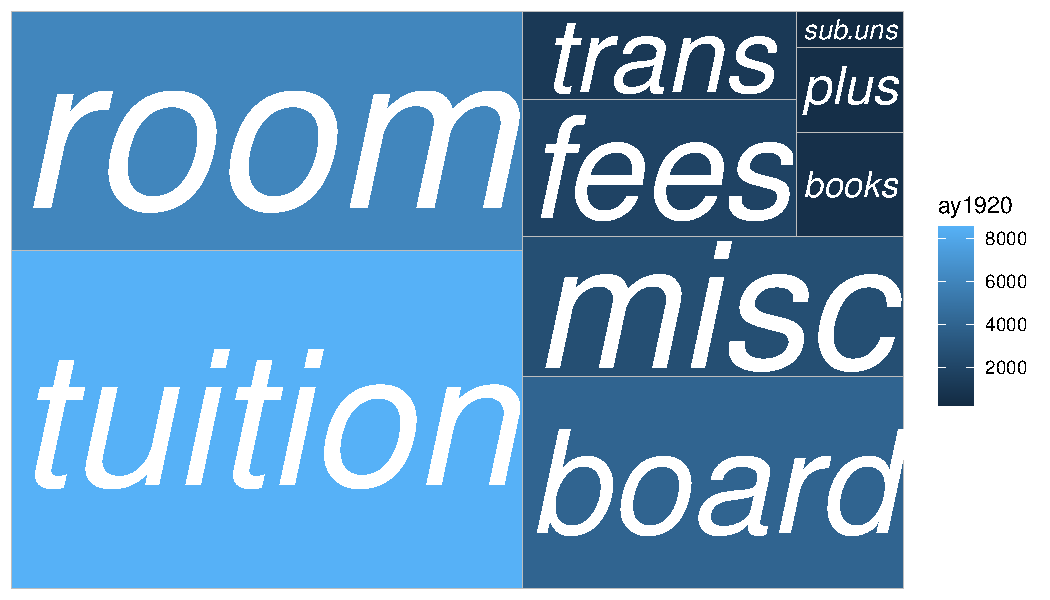
\includegraphics{02-COA_files/figure-latex/2.2.5-coa-res-1.pdf}

\hypertarget{financial-aid-awarded}{%
\chapter{Financial Aid Awarded}\label{financial-aid-awarded}}


\includegraphics[width=1\linewidth]{C:/Users/gfalk/Documents/BookdownPT/images/GEORGIA-XH-FC}

Undergraduate Cost of Attendance

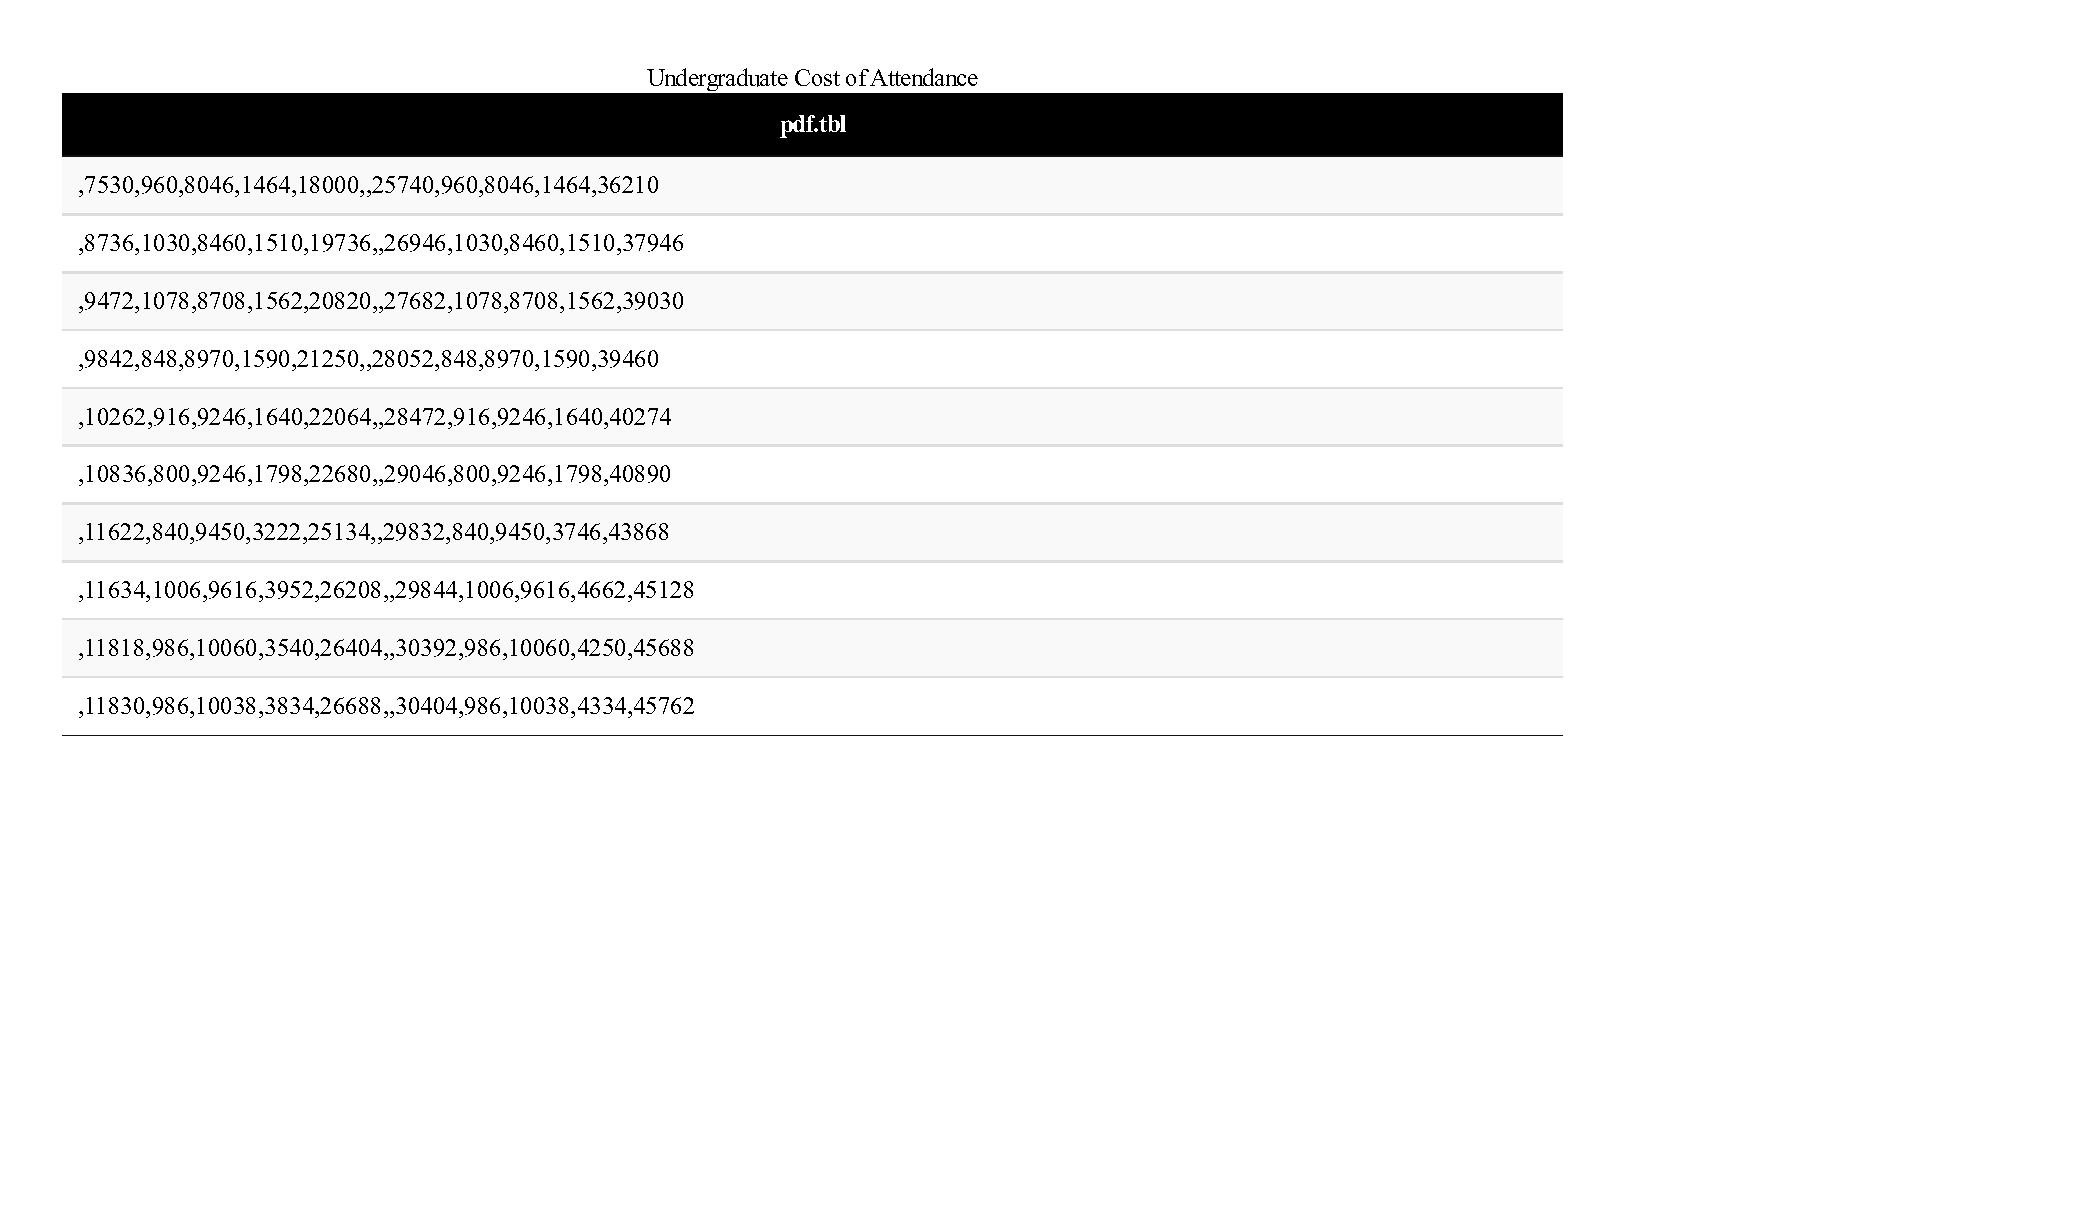
\includegraphics{03-Financial-Aid-Awarded_files/figure-latex/unnamed-chunk-1-1.pdf}

\begin{table}
\caption{(\#tab:2.o-UG-COA)Undergraduate Cost of Attendance Table}

\centering
\begin{tabular}[t]{r}
\toprule
x\\
\midrule
NA\\
7530\\
960\\
8046\\
1464\\
\addlinespace
18000\\
NA\\
25740\\
960\\
8046\\
\addlinespace
1464\\
36210\\
\bottomrule
\end{tabular}
\centering
\begin{tabular}[t]{r}
\toprule
x\\
\midrule
NA\\
8736\\
1030\\
8460\\
1510\\
\addlinespace
19736\\
NA\\
26946\\
1030\\
8460\\
\addlinespace
1510\\
37946\\
\bottomrule
\end{tabular}
\centering
\begin{tabular}[t]{r}
\toprule
x\\
\midrule
NA\\
9472\\
1078\\
8708\\
1562\\
\addlinespace
20820\\
NA\\
27682\\
1078\\
8708\\
\addlinespace
1562\\
39030\\
\bottomrule
\end{tabular}
\centering
\begin{tabular}[t]{r}
\toprule
x\\
\midrule
NA\\
9842\\
848\\
8970\\
1590\\
\addlinespace
21250\\
NA\\
28052\\
848\\
8970\\
\addlinespace
1590\\
39460\\
\bottomrule
\end{tabular}
\centering
\begin{tabular}[t]{r}
\toprule
x\\
\midrule
NA\\
10262\\
916\\
9246\\
1640\\
\addlinespace
22064\\
NA\\
28472\\
916\\
9246\\
\addlinespace
1640\\
40274\\
\bottomrule
\end{tabular}
\centering
\begin{tabular}[t]{r}
\toprule
x\\
\midrule
NA\\
10836\\
800\\
9246\\
1798\\
\addlinespace
22680\\
NA\\
29046\\
800\\
9246\\
\addlinespace
1798\\
40890\\
\bottomrule
\end{tabular}
\centering
\begin{tabular}[t]{r}
\toprule
x\\
\midrule
NA\\
11622\\
840\\
9450\\
3222\\
\addlinespace
25134\\
NA\\
29832\\
840\\
9450\\
\addlinespace
3746\\
43868\\
\bottomrule
\end{tabular}
\centering
\begin{tabular}[t]{r}
\toprule
x\\
\midrule
NA\\
11634\\
1006\\
9616\\
3952\\
\addlinespace
26208\\
NA\\
29844\\
1006\\
9616\\
\addlinespace
4662\\
45128\\
\bottomrule
\end{tabular}
\centering
\begin{tabular}[t]{r}
\toprule
x\\
\midrule
NA\\
11818\\
986\\
10060\\
3540\\
\addlinespace
26404\\
NA\\
30392\\
986\\
10060\\
\addlinespace
4250\\
45688\\
\bottomrule
\end{tabular}
\centering
\begin{tabular}[t]{r}
\toprule
x\\
\midrule
NA\\
11830\\
986\\
10038\\
3834\\
\addlinespace
26688\\
NA\\
30404\\
986\\
10038\\
\addlinespace
4334\\
45762\\
\bottomrule
\end{tabular}
\end{table}

\hypertarget{types-and-sources-of-aid.xls}{%
\chapter{Types and Sources of Aid.xls}\label{types-and-sources-of-aid.xls}}

Some \emph{significant} applications are demonstrated in this chapter.

\hypertarget{example-one}{%
\section{Example one}\label{example-one}}

\hypertarget{example-two}{%
\section{Example two}\label{example-two}}

\hypertarget{academic-year-student-financial-aid-awards-by-type}{%
\chapter{Academic Year Student Financial Aid Awards by Type}\label{academic-year-student-financial-aid-awards-by-type}}

We have finished a nice book.

  \bibliography{book.bib,packages.bib}

\end{document}
